\documentclass[10pt,a4paper]{article}

\usepackage[utf8]{inputenc}
\usepackage[T1]{fontenc}
\usepackage{amsmath,amssymb}
\usepackage{booktabs}
\usepackage{caption}
\usepackage{tabularx}
\usepackage{geometry}
\usepackage{graphicx}
\usepackage{hyperref}
\usepackage[round,authoryear]{natbib}

\geometry{margin=0.75in}
\captionsetup[table]{skip=3pt}
\captionsetup[figure]{skip=3pt}
\emergencystretch=1.5em
\setlength{\abovedisplayskip}{4pt}
\setlength{\belowdisplayskip}{4pt}
\graphicspath{{../../experiments/outputs/}}
\newcolumntype{Y}{>{\raggedright\arraybackslash}X}

\title{Bayesian Decision and Uncertainty:\\Asymmetric Clinical Triage for Skin Lesions}
\author{}
\date{}

\begin{document}

\maketitle
\vspace{-1.5em}

\begin{abstract}
\noindent Melanoma triage from dermoscopic images is not a symmetric classification problem: missing a melanoma is far costlier than referring a benign lesion. Using the binary melanoma-versus-benign task on HAM10000/ISIC 2018, we compare an HSV-histogram Gaussian mixture model (GMM) with an EfficientNet-B0 classifier under Monte Carlo (MC) Dropout, and study how calibration, asymmetric Bayesian loss, and epistemic uncertainty change triage behaviour. Averaged over three seeds on lesion-aware held-out splits, the calibrated deep model reaches AUC $0.858\pm0.002$ versus $0.796\pm0.009$ for the calibrated baseline (Brier $0.079$, ECE $0.019$). A $10{:}1$ false-negative to false-positive loss ratio gives about 87\% sensitivity at 66\% specificity; a calibration-selected 98\% sensitivity operating point reaches 98.9\% test sensitivity at 27\% specificity. Adding an MC Dropout uncertainty zone auto-reassures 19\% of lesions with, on average, 1--2 false negatives. Calibration and uncertainty, not accuracy alone, are what make an asymmetric triage policy safe to interpret.
\end{abstract}

\section{Introduction}
A classifier can rank melanomas well by AUC yet still be unsafe at the operating point used in deployment, because false negatives (missed melanoma) and false positives (unnecessary referral) are not equally costly: a missed melanoma risks delayed treatment of a potentially lethal disease, while an unnecessary referral costs anxiety and clinician time. This report asks how a melanoma-triage classifier should behave once that asymmetry, together with probability calibration and predictive uncertainty, is made explicit, using HAM10000 dermoscopic images in the ISIC 2018 context. Rather than treating melanoma detection as a plain binary-classification benchmark, we treat it as a Bayesian decision problem: the same predictions can imply very different clinical actions depending on the assumed cost ratio, on how well the predicted probabilities are calibrated, and on how confident the model is in each individual prediction.

\section{Related Work}
The ISIC 2018 challenge standardized evaluation of lesion classification across acquisition sources \citep{codella2018skin}, and HAM10000 addressed the prior scarcity of large, diagnostically varied dermoscopy datasets \citep{tschandl2018ham10000}. Most prior work on these benchmarks reports ranking metrics such as AUC or accuracy, which are agnostic to the asymmetric cost of clinical errors. EfficientNet provides a compact, strong ImageNet-pretrained backbone for the discriminative model \citep{tan2019efficientnet}, and is used here in place of a classical hand-crafted feature pipeline to test how much a learned representation improves on a simple colour-histogram baseline. Because raw network outputs are often over-confident, we rely on post-hoc calibration and expected calibration error (ECE) as in \citet{guo2017calibration} to make probabilities usable for a cost-sensitive decision rule, and use MC Dropout \citep{gal2016dropout} as a lightweight estimate of epistemic uncertainty, rather than a full Bayesian neural network.

\section{Technical Information}
\textbf{Task.} Melanoma (\texttt{mel}) is the positive class; nevi, benign keratoses, dermatofibroma, and vascular lesions are pooled as benign negatives (9{,}174 images total, 12.1\% melanoma). Basal cell carcinoma and actinic keratoses are excluded so that referring them is never scored as an error. Splits are grouped by \texttt{lesion\_id} (no lesion appears in two partitions) and stratified into fit/validation/calibration/test folds ($\approx$52/12/16/20\%).

\noindent \textbf{Models.} The baseline extracts global HSV colour histograms and fits one Gaussian mixture per class (BIC-selected components), converted to a posterior via Bayes' rule. The deep model fine-tunes an EfficientNet-B0 backbone with a single logistic output, trained with unweighted binary cross-entropy so the raw sigmoid output stays interpretable as a probability estimate.

\noindent \textbf{Calibration and decision rule.} Both models are Platt-scaled on a held-out calibration split and scored with Brier score and ECE. Predicted probabilities feed a Bayesian decision rule: referring a lesion is preferred over auto-reassurance whenever $\hat p\,L_{FN} > (1-\hat p)\,L_{FP}$, i.e.\ above threshold $\tau = L_{FP}/(L_{FP}+L_{FN})$. For a $10{:}1$ cost ratio, $\tau \approx 0.091$.

\noindent \textbf{Uncertainty.} MC Dropout keeps dropout active at inference, giving $T=30$ stochastic probabilities per image. Their mean is used for thresholding; predictive entropy and mutual information (dropout disagreement) flag lesions that should go to manual review rather than be treated as ordinary confident predictions.

\section{Results}
The deep model discriminates better than the colour-only baseline (AUC $0.858\pm0.002$ vs.\ $0.796\pm0.009$) and is more stable across seeds, as shown by the ROC curves in Figure~\ref{fig:roc}. Calibration is good: test Brier $0.079\pm0.006$, ECE $0.019\pm0.006$ (down from raw ECE $0.026\pm0.009$), which matters because an uncalibrated model can satisfy a nominal Bayesian threshold while still misrepresenting the true risk of referral or auto-reassurance. At the symmetric $\tau=0.5$ threshold, sensitivity is only 21.7\%, which is clinically unacceptable; asymmetric thresholds trade specificity for sensitivity as shown in Table~\ref{tab:results}. The theoretical $10{:}1$ threshold still misses on average 27 of the roughly 200 melanomas in the test split, which motivates choosing the threshold directly from a target sensitivity instead. Table~\ref{tab:operating} selects thresholds on the calibration split for minimum sensitivity and evaluates them once on the held-out test split: a 98\% sensitivity target reaches 98.9\% test sensitivity at 27.1\% specificity, at the cost of referring 76\% of lesions.

\begin{figure}[htbp]
\centering
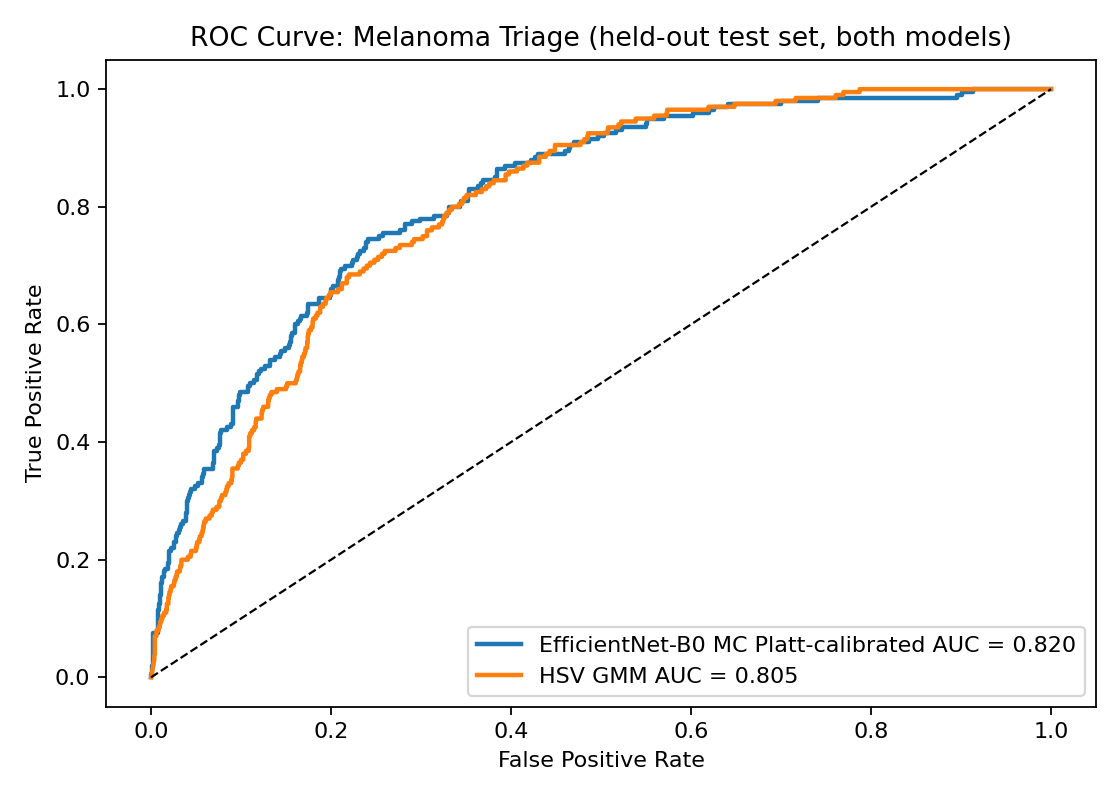
\includegraphics[width=0.58\textwidth]{roc_curve_triage.png}
\caption{ROC curves for the Platt-calibrated deep model and the HSV GMM baseline (primary seed, held-out test split).}
\label{fig:roc}
\end{figure}

\begin{table}[htbp]
\centering
\caption{Held-out test triage metrics, deep model, mean (sd) over three seeds.}
\label{tab:results}
\small
\begin{tabular}{lrrrr}
\toprule
Threshold rule & Sensitivity & Specificity & Referral & FN \\
\midrule
Symmetric ($\tau=0.5$) & 0.217 (0.023) & 0.984 (0.002) & 0.039 (0.004) & 168 (20) \\
$10{:}1$ loss ratio & 0.873 (0.031) & 0.656 (0.036) & 0.405 (0.037) & 27 (5) \\
$20{:}1$ loss ratio & 0.944 (0.004) & 0.517 (0.046) & 0.536 (0.044) & 12 (2) \\
\bottomrule
\end{tabular}
\end{table}

\begin{table}[htbp]
\centering
\caption{Sensitivity-constrained thresholds, selected on the calibration split and evaluated on the held-out test split.}
\label{tab:operating}
\small
\begin{tabular}{lrrrr}
\toprule
Target sensitivity & Test sensitivity & Specificity & Referral & FN \\
\midrule
0.95 & 0.964 (0.044) & 0.451 (0.010) & 0.596 (0.044) & 8 (2) \\
0.98 & 0.989 (0.035) & 0.271 (0.038) & 0.760 (0.028) & 2 (1) \\
0.99 & 0.993 (0.029) & 0.214 (0.034) & 0.810 (0.028) & 1 (1) \\
\bottomrule
\end{tabular}
\end{table}

Combining the 99\%-sensitivity threshold with an MC Dropout mutual-information cutoff (95th percentile on the calibration split) yields a three-zone policy: lesions with low predicted probability and low uncertainty are auto-reassured, high-probability lesions are referred urgently, and the remainder go to manual review. Table~\ref{tab:triage-zone} summarizes this policy on the held-out test split.

\begin{table}[htbp]
\centering
\caption{Three-zone triage policy using calibrated probability and MC Dropout mutual information, mean (sd) over three seeds.}
\label{tab:triage-zone}
\small
\begin{tabular}{lrr}
\toprule
Triage zone & Share of lesions & Other metrics \\
\midrule
Auto-reassured & 19.0\% (2.8\%) & 1.3 (0.9) FN; 99.3\% (0.5\%) sensitivity after \\
Manual review & 77.1\% (2.6\%) & -- \\
Urgent referral & 3.9\% (0.4\%) & 64.4\% (0.4\%) precision \\
\bottomrule
\end{tabular}
\end{table}

\section{Discussion and Conclusion}
Better ranking (AUC) does not by itself solve the clinical problem: the Bayesian threshold shows that a usable operating point depends on calibration quality and an explicit loss ratio, and even the calibrated $10{:}1$ threshold still misses about 13\% of melanomas. Sensitivity-constrained thresholds make the safety tradeoff explicit at the cost of a high referral burden (76--81\% referral for 98--99\% sensitivity), which is a more honest way to communicate the operating point than reporting AUC or accuracy alone. MC Dropout uncertainty adds a third option beyond refer/auto-reassure: routing ambiguous, high-disagreement lesions to manual review lets the auto-reassured group reach 99.3\% sensitivity while keeping urgent referrals enriched for melanoma, so uncertainty is used as an input to the decision rather than only reported as a diagnostic plot.

Several limitations temper these conclusions. HAM10000 is retrospective, multi-source, and partly labelled without histopathology \citep{tschandl2018ham10000}, and similar benchmark scores can still correspond to different generalization behaviour on external data \citep{codella2018skin}. Our calibration and threshold-selection splits are internal to the same HAM10000 pool, and three random seeds quantify internal split variability but not external validity. The GMM baseline is deliberately simple and is only a check on how much signal colour alone provides. The results should be read as a controlled demonstration of Bayesian triage behaviour, not as evidence of clinical readiness.

In summary, asymmetric melanoma triage cannot be reduced to maximizing accuracy or AUC. A usable system must rank lesions, produce calibrated probabilities, and expose epistemic uncertainty, so that an explicit cost ratio or sensitivity target can be translated into a referral policy with a known, quantified referral burden and false-negative rate.

\bibliographystyle{plainnat}
\bibliography{skin_lesion_triage_refs}

\end{document}
